% \iffalse
\let\negmedspace\undefined
\let\negthickspace\undefined
\documentclass[journal,12pt,twocolumn]{IEEEtran}
\usepackage{cite}
\usepackage{amsmath,amssymb,amsfonts,amsthm}
\usepackage{algorithmic}
\usepackage{graphicx}
\usepackage{textcomp}
\usepackage{xcolor}
\usepackage{txfonts}
\usepackage{listings}
\usepackage{enumitem}
\usepackage{mathtools}
\usepackage{gensymb}
\usepackage{circuitikz}
\usepackage{comment}
\usepackage[breaklinks=true]{hyperref}
\usepackage{tkz-euclide}
\usepackage{listings}
\usepackage{gvv}
\def\inputGnumericTable{}
\usepackage[latin1]{inputenc}
\usepackage{color}
\usepackage{array}
\usepackage{longtable}
\usepackage{calc}
\usepackage{multirow}
\usepackage{hhline}
\usepackage{ifthen}
\usepackage{lscape}

\newtheorem{theorem}{Theorem}[section]
\newtheorem{problem}{Problem}
\newtheorem{proposition}{Proposition}[section]
\newtheorem{lemma}{Lemma}[section]
\newtheorem{corollary}[theorem]{Corollary}
\newtheorem{example}{Example}[section]
\newtheorem{definition}[problem]{Definition}
\newcommand{\BEQA}{\begin{eqnarray}}
\newcommand{\EEQA}{\end{eqnarray}}
\newcommand{\define}{\stackrel{\triangle}{=}}
\theoremstyle{remark}
\newtheorem{rem}{Remark}
\begin{document}

\bibliographystyle{IEEEtran}
\vspace{3cm}

\title{GATE -BM 16}
\author{EE23BTECH11057 - Shakunaveti Sai Sri Ram Varun$^{}$% &lt;-this % stops a space
}
\maketitle
\newpage
\bigskip
\vspace{2cm}
\textbf{Question: }
For the circuit given below, choose the angular frequency $ \omega_0$ at which voltage across capacitor has maximum amplitude?\\\\
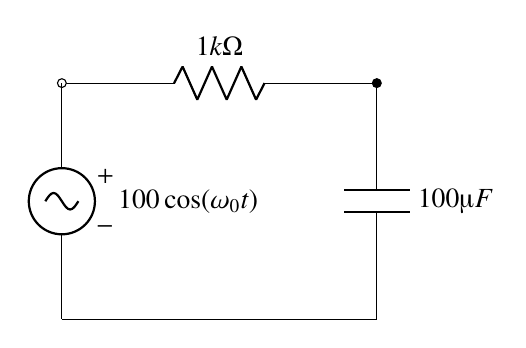
\begin{tikzpicture}
\centering
    \draw (0,0) to[R, l=$1k\ohm$, o-*] (4,0);
    \draw (4,0) to[C, l=$100\micro F$] (4,-3);
    \draw (0,0) to[sV, v=$100\cos(\omega_0 t)$, american] (0,-3);
    \draw (0,-3)--(4,-3);
\end{tikzpicture}\\\\
\textbf{Solution}:\\
\begin{table}[htbp] 
\centering
\begin{tabular}{|c|c|c|}
    \hline
    \textbf{Parameter} & \textbf{Description} & \textbf{Value} \\
    \hline
    $x\brak{0}$ & First term of G.P. & 3 \\
    \hline
    $r$ & common ratio of G.P. & r \\
    \hline
\end{tabular}


\caption{input values}
\label{tab: table-bm16}
\end{table}
Writing differential equation for circuit,
\begin{align}
V_i\brak{t} &= V_r\brak{t} + V_c\brak{t}\\
V_i\brak{t} &= 10^{-1}\frac{dV_c\brak{t}}{dt} + V_c\brak{t}
\end{align}
Writing in s-domain (Laplace transform)
\begin{align}
L[V_i\brak{t}] &= L[10^{-1}\frac{dV_c\brak{t}}{dt}] + L[V_c\brak{t}]\\
V_i\brak{s} &= 10^{-1}V_c\brak{s}s + V_c\brak{s}\\
\therefore V_c\brak{s} &= \frac{1000s}{\brak{s^2+ \omega_o^2}}\frac{1}{(s+10)}
\end{align}
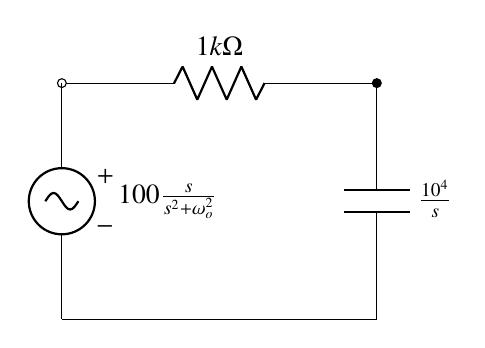
\begin{tikzpicture}
\centering
    \draw (0,0) to[R, l=$1k\ohm$, o-*] (4,0);
    \draw (4,0) to[C, l=$\frac{10^4}{s}$] (4,-3);
    \draw (0,0) to[sV, v=$100\frac{s}{s^2+\omega_o^2}$, american] (0,-3);
    \draw (0,-3)--(4,-3);
\end{tikzpicture}\\\\
splitting $ V_c\brak{s}$ into partial fractions,
\begin{align}
V_c\brak{s} &= \frac{10^4s+10^3\omega_o^2}{\brak{10^2+\omega_o^2}\brak{s^2+\omega_o^2}}-\frac{10^4}{\brak{s+10}\brak{10^2+\omega^2}}
\end{align}
on applying inverse Laplace transform,
\begin{align}
V_c\brak{t}&= \frac{10^4cos(\omega_o t)}{10^2+\omega_o^2}+\frac{10^3\omega_osin(\omega_o t)}{10^2+\omega_o^2}-\frac{10^4e^{-10t}}{10^2+\omega_o^2}
\end{align}
\vspace{5cm}
last term is natural response, we can ignore it.\\
Now, the amplitude can be computed by,
\begin{align}
|V_c\brak{t}| &= \frac{10^3}{\sqrt{10^2+\omega_o^2}}
\end{align}
we can see the highest amplitude is obtained when $ \omega_o = 0$.
\end{document}
